\section{Introducing SPIND}

We will now discuss our proposed algorithm $SPIND$, which stands for \textbf{s}calable \textbf{p}artial \textbf{in}clusion \textbf{d}ependencies. Further the german word $Spind$ is a special kind of closet and often multiple "Spinds" are placed next to each other. This is a metaphor to the algorithms procedure. Every input relation will be transformed to a "Spind" of sorted values with connected attributes (attribute combinations), which is surely bigger than a $BINDER$ bucket, but there are far fewer "Spinds" than $BINDER$ would create buckets.

\begin{figure}[h]
    \centering
    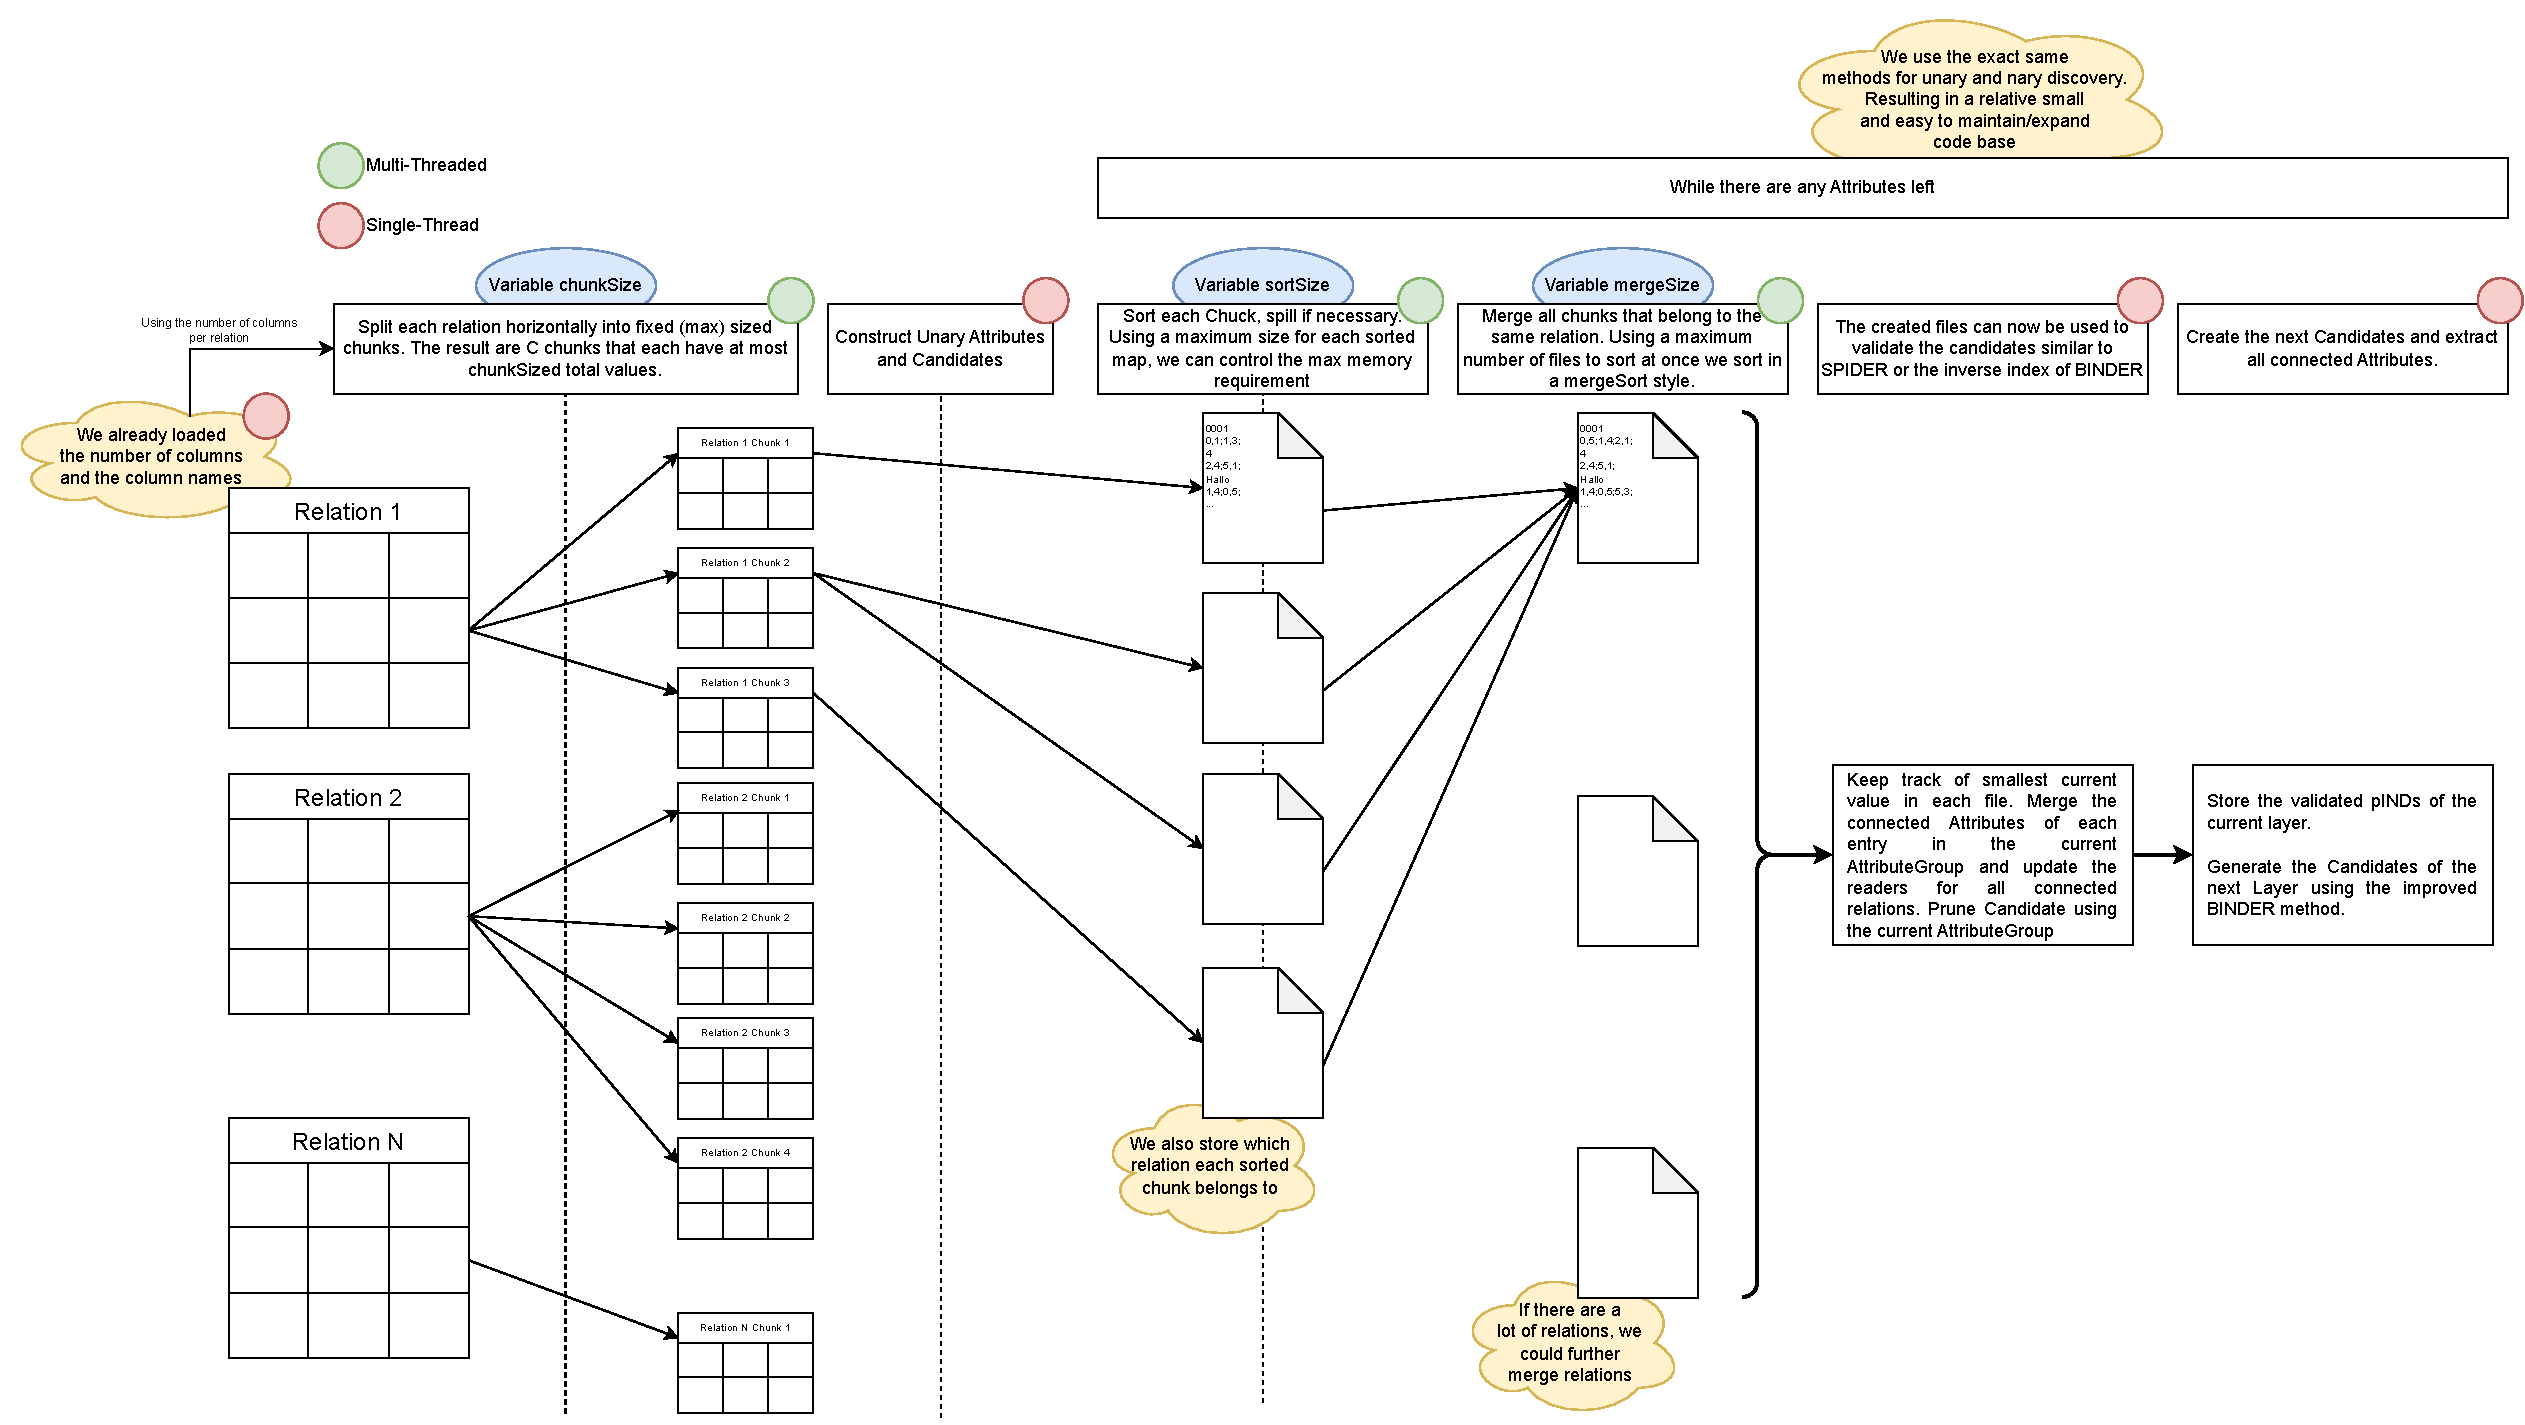
\includegraphics[width=0.99\textwidth]{files/SPIND.pdf}
    \caption{Conceptual overview of \textit{SPIND}}
    \label{fig:spind}
\end{figure}

\subsection{Chunking the input relations}
Modern CPUs feature multiple cores capable of executing tasks concurrently. Previous studies have largely overlooked the potential of multi-threading. In contrast, $SPIND$ will leverage multi-threading extensively to maximize hardware utilization. Achieving this objective necessitates the identification of independent tasks capable of being processed in parallel. \\

\noindent The execution starts by fetching some very basic information about the input relations. For each relational instance (input table) $SPIND$ will extract the header column (if present) and store the number of columns each table has. Using a constant $CHUNK\_SIZE$ which is set by the user, we spilt each relation into somewhat equal parts. Each chunk will consist of at most $\lfloor \frac{CHUNK\_SIZE}{\# cloumns \: in \: relation} \rfloor$ rows. The complexity of processing a relation directly correlates to the number of total values in that relation. While this may be an oversimplification since there are many more factors, like the distribution of duplicate values, the raw size is easy to modify and a heuristic that can be applied without any specific dataset knowledge. Each of the resulting chunks is associated with exactly one relation and carries a subset of that relations rows. \\

\noindent Chunking is done exactly once at the very start and is not repeated for n-ary layers. We reuse the same chunks in every layer of the n-ary pIND discovery. \\
% TODO Link section discussing chunking effectiveness.

\noindent Since $SPIND$ almost always operates on the relation layer, a hash based partitioning, similar to $BINDER$, is not feasible. For the validation, we need to descend to the attribute layer and there we need to know which attributes (attribute combinations) share at least one value. A partitioning would therefore be required to split the dataset into $n$ groups $G_1, \dots, G_n$ such that for every tuple of values $t_i$ generate by some row, it holds that if $t_i \in G_j$ than 
\begin{itemize}
    \item[1)] $\forall \: t_k \in G \setminus G_j : t_i \cap t_k = \emptyset$
    \item[2)] $t_i \cap t_k \not = \emptyset \: \forall t_k \in G_j$
\end{itemize}
To find such groups we would need knowledge of all values in a relation. Even if we expand the groups row by row and merge when necessary, solving this grouping problem would create a lot of new complexity. To still understand the potential benefit, table 

\begin{table}
    \label{tab:partitioning}
    \begin{tabular}{c|c|c|c|c} 
     dataset & average & median & min & max\\ 
     \hline\hline
     data.gov & - & - & - & -\\ 
     \hline
     musicbrainz & - & - & - & -\\
    \end{tabular}
    \caption{Possible partitions during u-nary discovery on a relational level.}
\end{table}

\subsection{Probabilistic Filtering}
Assume we would know the set of all values, which only occur in referred attributes. Such a set could be used to filter the values that would need to be sorted, merged and validated. How the filter is filled and where exactly it is used will be discussed in the sorting and validation sections. This section will explain the reason why such a filter can be used in the first way and which benefits it brings.

Given two projections $r_1[X]$ and $r_2[Y]$ and the candidate $r_1[X] \subseteq_\rho r_2[Y]$ than we can trivially see that placing $r_2[Y]$ into the calculation will always yield the same result as placing $r_2[Y] \setminus \text{\{ref only values\}}$ into the equation.

Since we may not be able to actually keep all of the values in main memory, we need a different approach of filtering the values. An important observation being, that we need to be certain, that all values which are present in at least one dependant attribute need to make it through the filter. If values which are only in dependant (or irrelevant) attributes make it through the filter, that creates more computational complexity, but will not create any incorrect results.

These constraints can be full filled by build a probabilistic filter in which all values that appear in an dependant attribute at least once are stored. Such a filter can than be queried using a value to check if that value was added. If the value was added previously it will always return true. If the values was not added it may create a false positive at a rate of typically less than 5\%. There are multiple options for such filters.

Research regarding probabilistic data structures focuses on two primary metrics govern research evaluation: the computational efficiency of insertion and query operations, and the required number of bits for storing individual values within the structure\cite{fan2014cuckoo}. Bloom filters are initialized with an anticipated number of elements and a target false positive rate. However, if additional values are incorporated beyond the initial expectation, Bloom filters may become oversaturated, leading to an approaching false positive rate of 1 \cite{tarkoma2011theory}. Bloom filters use about 44\% ($log_2(e)$) more space per key than the theoretical lower bound. There are probabilistic data structures which are closer to the theoretical lower bound, but these structures impose more complex strategies which are out of scope of this thesis \cite{fan2014cuckoo}.

The size of the Bloom Filter is set to 100 million expected values with a false positive rate of 1\% by default. With these settings the filter will consume TODO bytes of main memory. If the avilable memory is very limited, the filter should be initialized with a smaller size or higher false positive rate. Table \ref{tab:filter} shows how many values are inserted into the bloom filter during u-nary pIND discovery for each dataset. In section \ref{sec:spind_val} we will discuss in detail how the values are inserted into the filter.

\begin{table}
    \label{tab:filter}
    \begin{tabular}{c|c} 
     dataset & values in filter\\ 
     \hline\hline
     data.gov & - \\ 
     \hline
     musicbrainz & - \\
    \end{tabular}
    \caption{The number of items that are inserted into the bloom filter for each dataset.}
\end{table}


\subsection{Sorting Chunks}
% IDEA: spill based on occurrences to that point.
Our objective is to arrange each chunk in sorted order, a prerequisite for subsequent merging and validation procedures. Consistently, each chunk undergoes identical processing steps, executed concurrently.

We employ a $CSVReader$ instance for each chunk, specifying the relevant attribute combinations. Subsequently, line-by-line processing of the chunk occurs, with the concurrent update of associated attributes to their latest values after each line is read. To manage these values and their associations, we employ a hash based mapping structure where values are mapped to their respective attributes along with the frequency of occurrences, thus forming a nested map. However, to prevent memory overflow, we constrain the size of this map using a constant denoted as $SORT\_SIZE$. When the map size reaches this threshold or when sorting is complete, data is spilled to disk. This storage process will first sort the key set of the outer map. Subsequently, each entry is iterated over in sorted order, with each value persisted on one line followed by its associated attributes in a specific pattern: $"attributeId_1,occurrences_1;attributeId_2,occurrences_2;\dots;"$. Figure \ref{fig:sorting} illustrates this workflow. For every spilled file, we retain the path of the sorted (sub) chunk, ultimately returning a list of these paths. \\

An optimization we can conduct here is spilling values based on the sum of occurrences in the connected values. We know that in a single chunk, there are at most \textit{CHUNK\_SIZE} unique values. In n-ary layers there might be relations where the number candidates of than relation is greater than the number of columns. Therefor we can calculate that the maximal possible number of distinct values generated from a chunk is $N = \underbrace{\lfloor \frac{CHUNK\_SIZE}{\#cloumns} \rfloor}_{= \#rows} \cdot \#candidates$, since every row can produce at most one unique value for each candidate. We can now say that $\frac{N}{SORTED\_SIZE}$ is the biggest possible minimum of occurrences over all present values. The proposed heuristic suggests to keep all values with more than $\frac{\#candidates \cdot CHUNK\_SIZE}{SORTED\_SIZE}$ occurrences which is greater than $\frac{N}{SORTED\_SIZE}$ in main memory and only spill those values which where not seen often. The idea being, that values which have occurred often will be more likely to occur often. Spilling these last can save complexity during merging since less candidate occurrences need to be deserialized.

\begin{figure}[h]
    \centering
    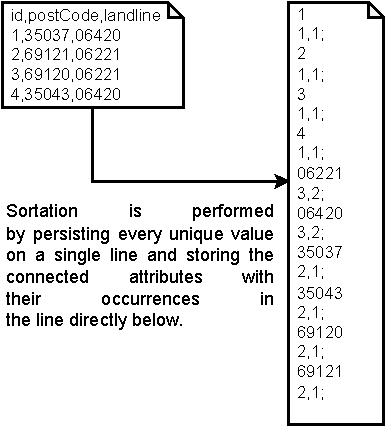
\includegraphics[width=0.45\textwidth]{files/Sorting.pdf}
    \caption{Simplified illustration of the sorting process.}
    \label{fig:sorting}
\end{figure}

\subsection{Merging (spilled) Chunks}
We now have a bunch of files which are all sorted by themselves. The next step is to merge all the files with originated from the same relation. Again, this is computed in parallel. To avoid too many files being opened at the same time the constant $MERGE\_SIZE$ can be used to limit the number of files which are being sorted per thread. Due to multithreading the actual number of simultaneously opened files is $\#threads \cdot (MERGE\_SIZE + 1)$. The plus one originates since we always need to open the resulting output file of a merge as well.
% TODO decide on default and perform experiments

\subsection{Validation}\label{sec:spind_val}
The validation process expects a sorted file per relation. The whole idea of the process works analog to the validation performed by \textit{SPIDER}. Given the sorted files we check which attributes (attribute combinations) share value and move the readers forward bit by bit in a way that only those readers are updated which share the same smallest value. \textit{SPIDER} uses a priority queue which stores the head value of each reader. Such a data structure enables us to calculate the smallest of the head values in $log(M)$ time, $M$ being the number of attributes (attribute combinations). Assume the complexity of pruning the connected attributes to some value is $O(k)$. Validating all values $N$ would cost $O(k \cdot N \cdot log(M))$. Pruning is a synchronous task, meaning the active candidates need to be synchronized between every prune. We will therefor try to create the attribute groups in parallel and conduct pruning in the main thread.

